\chapter{Turing Machine}
\label{ch-turing}

\newcommand{\TA}[0]{\Sigma^+}

This chapter is based on Ref.\cite{wiki-turing-machine}.

In this chapter, we define a {\bf Turing Machine} (TM) as
 a generalization
of a special case of a Petri net called a Finite
State Machine (FSM).
Petri nets are discussed in Chapter \ref{ch-petri}. FSM are discussed
in Chapter \ref{ch-finite-state}. We will assume
that the reader has read those two chapters before tackling this one.

Fig.\ref{fig-turing-phsical} presents an idealized physical model
of a TM.
It consists of a 
\begin{itemize}
\item
a {\bf tape}. The tape is infinite in both directions,
and separated into tape cells,
but only a finite number of tape cells may be non-blank.
Each non-blank cell contains one symbol from a pre-defined set of symbols called the tape alphabet.
\item
a {\bf head}
that is one tape cell wide. It moves, relative to the tape,  from one tape cell, 
to the cell immediately to its right or to its left.
The head can read the value of the symbol under it and replace
it (write) by another symbol.
\item a {\bf control/memory} unit that remembers 
the current place/state ($\rvp_2$ in Fig.\ref{fig-turing-phsical})
\end{itemize}

\begin{figure}[h!]
\centering
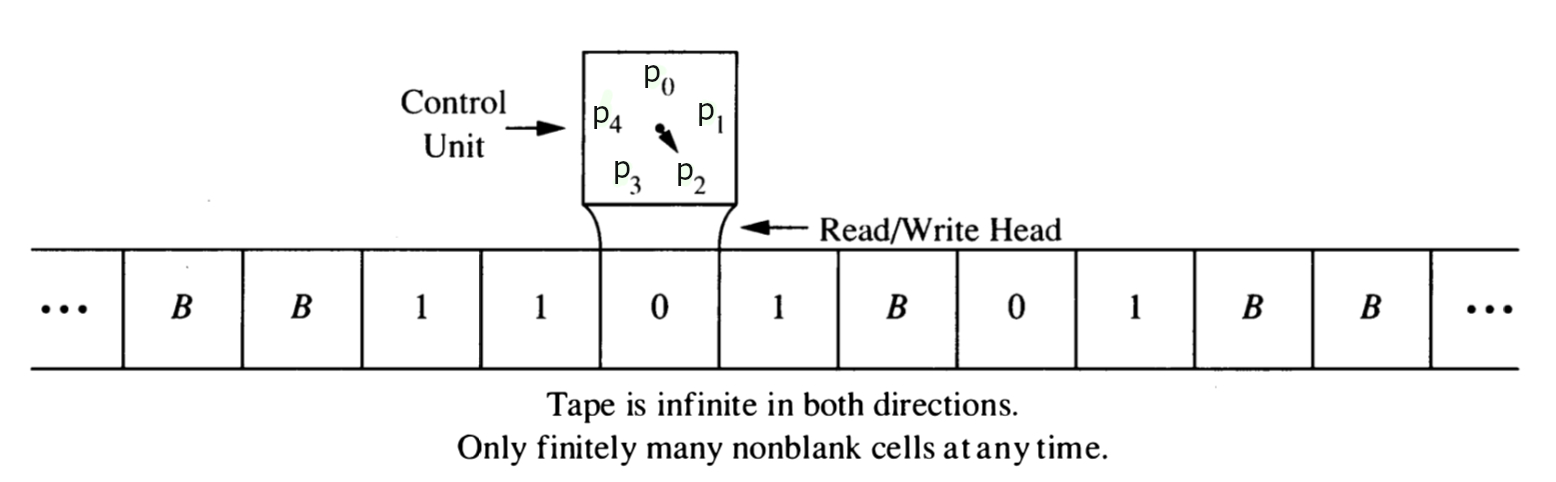
\includegraphics[width=6in]
{turing/turing-physical.jpg}
\caption{Idealized physical model of Turing Machine.}
\label{fig-turing-phsical}
\end{figure}

\section{Example}

\begin{figure}[h!]
$$
\begin{array}{cc}
\xymatrix@C=6pc@R=3pc{
\PinkCircle{\rva}
\ar[rr]|{\rvx_1=(0,1,R)}
\ar[rd]|{\rvx_3=(1,1, L)}
&&\Circle{\rvb}\ar@(ru,lu)[]_{\rvx_6=(1,1,R)}
\ar@/_2pc/[ll]|{\rvx_2=(0,1,L)}
\\
\ar[u]
&\Circle{\rvc}
\ar[ru]|{\rvx_4=(0,1, L)}
\ar[r]|{\rvx_5=(1,1, R)}
&\DCircle{\rvh}
}
&
\begin{array}{c|c|c|}
\rvp\rarrow \rvx
&\ket{\rvp'}=\rvx\ket{\rvp}
& \lam=(\lam_r,
\lam_w,
\lam_m)
\\
\hline\hline
\rva\rarrow\rvx_1
&\rvb
&(0,1,R)
\\ \hline
\rvb\rarrow\rvx_2
&\rva
&(0,1,L)
\\ \hline
\rva\rarrow\rvx_3
&\rvc
& (1,1,L)
\\ \hline
\rvc\rarrow\rvx_4
&\rvb
& (0,1,L)
\\\hline
\rvc\rarrow\rvx_5
&\rvh
&(1,1,R)
\\ \hline
\rvb\rarrow\rvx_6
&\rvb
&(1,1,R)
\\ \hline
\end{array}
\end{array}
$$
\caption{The \qt{3-state Busy Beaver} Turing machine represented as a FSM Petri net.}
\label{fig-3-state-bb}
\end{figure}


\begin{table}[h!]
\begin{tabular}{lllllllllll}
1 &  &  &  &  & $\rva$ &  &  &  &  &  
\\ \hline
\multicolumn{1}{|l|}{\cellcolor[HTML]{FFFFC7}0} 
& \multicolumn{1}{l|}{0} 
& \multicolumn{1}{l|}{\cellcolor[HTML]{FFFFC7}0} 
& \multicolumn{1}{l|}{0} 
& \multicolumn{1}{l|}{\cellcolor[HTML]{FFFFC7}0} 
& \multicolumn{1}{l|}{\ul{0}} 
& \multicolumn{1}{l|}{\cellcolor[HTML]{FFFFC7}0} 
& \multicolumn{1}{l|}{0} 
& \multicolumn{1}{l|}{\cellcolor[HTML]{FFFFC7}0} 
& \multicolumn{1}{l|}{0} 
& \multicolumn{1}{l|}{\cellcolor[HTML]{FFFFC7}0} 
\\ \hline
\end{tabular}
\\
\begin{tabular}{lllllllllll}
2 &  &  &  &  &  & $\rvb$ &  &  &  &  
\\ \hline
\multicolumn{1}{|l|}{\cellcolor[HTML]{FFFFC7}0} 
& \multicolumn{1}{l|}{0} 
& \multicolumn{1}{l|}{\cellcolor[HTML]{FFFFC7}0} 
& \multicolumn{1}{l|}{0} 
& \multicolumn{1}{l|}{\cellcolor[HTML]{FFFFC7}0} 
& \multicolumn{1}{l|}{1} 
& \multicolumn{1}{l|}{\cellcolor[HTML]{FFFFC7}\ul{0}} 
& \multicolumn{1}{l|}{0} 
& \multicolumn{1}{l|}{\cellcolor[HTML]{FFFFC7}0} 
& \multicolumn{1}{l|}{0} 
& \multicolumn{1}{l|}{\cellcolor[HTML]{FFFFC7}0} 
\\ \hline
\end{tabular}
\\
\begin{tabular}{lllllllllll}
3 &  &  &  &  & $\rva$ &  &  &  &  &  
\\ \hline
\multicolumn{1}{|l|}{\cellcolor[HTML]{FFFFC7}0} 
& \multicolumn{1}{l|}{0} 
& \multicolumn{1}{l|}{\cellcolor[HTML]{FFFFC7}0} 
& \multicolumn{1}{l|}{0} 
& \multicolumn{1}{l|}{\cellcolor[HTML]{FFFFC7}0} 
& \multicolumn{1}{l|}{\ul{1}} 
& \multicolumn{1}{l|}{\cellcolor[HTML]{FFFFC7}1} 
& \multicolumn{1}{l|}{0} 
& \multicolumn{1}{l|}{\cellcolor[HTML]{FFFFC7}0} 
& \multicolumn{1}{l|}{0} 
& \multicolumn{1}{l|}{\cellcolor[HTML]{FFFFC7}0} 
\\ \hline
\end{tabular}
\\
\begin{tabular}{lllllllllll}
4 &  &  &  & $\rvc$ & &  &  &  &  &  
\\ \hline
\multicolumn{1}{|l|}{\cellcolor[HTML]{FFFFC7}0} 
& \multicolumn{1}{l|}{0} 
& \multicolumn{1}{l|}{\cellcolor[HTML]{FFFFC7}0} 
& \multicolumn{1}{l|}{0} 
& \multicolumn{1}{l|}{\cellcolor[HTML]{FFFFC7}\ul{0}} 
& \multicolumn{1}{l|}{1} 
& \multicolumn{1}{l|}{\cellcolor[HTML]{FFFFC7}1} 
& \multicolumn{1}{l|}{0} 
& \multicolumn{1}{l|}{\cellcolor[HTML]{FFFFC7}0} 
& \multicolumn{1}{l|}{0} 
& \multicolumn{1}{l|}{\cellcolor[HTML]{FFFFC7}0} 
\\ \hline
\end{tabular}
\\
\begin{tabular}{lllllllllll}
5 &  &  & $\rvb$ & & &  &  &  &  &  
\\ \hline
\multicolumn{1}{|l|}{\cellcolor[HTML]{FFFFC7}0} 
& \multicolumn{1}{l|}{0} 
& \multicolumn{1}{l|}{\cellcolor[HTML]{FFFFC7}0} 
& \multicolumn{1}{l|}{\ul{0}} 
& \multicolumn{1}{l|}{\cellcolor[HTML]{FFFFC7}1} 
& \multicolumn{1}{l|}{1} 
& \multicolumn{1}{l|}{\cellcolor[HTML]{FFFFC7}1} 
& \multicolumn{1}{l|}{0} 
& \multicolumn{1}{l|}{\cellcolor[HTML]{FFFFC7}0} 
& \multicolumn{1}{l|}{0} 
& \multicolumn{1}{l|}{\cellcolor[HTML]{FFFFC7}0} 
\\ \hline
\end{tabular}
\caption{First five steps of Busy Beaver TM 
defined by Fig.\ref{fig-3-state-bb}. }
\label{tab-busy-beaver}
\end{table}

Fig.\ref{fig-3-state-bb} shows an example of
a TM represented as a FSM Petri net. Everything in this diagram
should be familiar to the reader after reading the chapters
on pnets and FSM, except for the
transition  labelling function $\lam()$.

Whereas $\lam$ is a scalar (i.e., an element of the alphabet $\Sigma$)
for a FSM, for a TM it's a triple $(\lam_r, \lam_w, \lam_m)$.
$\lam_r$ is the tape symbol read, $\lam_w$
is the tape symbol written (after erasing the 
previous one). $\lam_m\in\{R, L\}$
commands the head to move one cell to the right (R)
or to the left (L).

Table \ref{tab-busy-beaver} gives the first five 
steps of the  Busy Beaver.

For the Busy Beaver example:

$\rvh=HALT$

$\calp= \{\rva, \rvb, \rvc, \rvh\}$  

$0=$ blank symbol

$\TA =\{0,1\}$, 

$\Sigma = \{1\}$

$\rvp(0)=\rva$

$\calp_{acc} =\{\rvh \}$




\section{Precise Definition}

\hrule
Same as in FSM:

$\calx =\{\rvx_i\}_{i=1}^{nx}$ are the {\bf transition nodes} of the pnet.

$\calp =\{\rvp_i\}_{i=1}^{np}$ are the {\bf place (or state) nodes} of the pnet.

$\rvp(0)\in \calp$, {\bf starting/initial place }

$\calp_{acc}\subset \calp$ are the 
{\bf acceptor/final places}. 

$\Delta:\calx\times\calp\rarrow \calp$ is the 
{\bf transition function}
\hrule
New for TM

$HALT\in \calp_{acc}$

$\TA =$ {\bf tape alphabet}

$B\in \TA$ is the  symbol for a {\bf blank space}.

$\Sigma=$ {\bf input alphabet}. $\Sigma\subset\TA-\{B\}$. 
This is the set of symbols other than $B$ that occur in the 
initial tape.

$\lam_{r}:\calx\rarrow \TA$ is the {\bf read  labelling function}

$\lam_{w}:\calx\rarrow \TA$ is the {\bf write  labelling function}

$\lam_{m}:\calx\rarrow \{L,R\}$ is the {\bf move 
labelling function} $L=$move Left, $R=$move Right. Some machines use $\{L,R,N\}$
as the range of $\lam_m$. $N$ is the command \qt{No movement}.

$\lam = (\lam_r, \lam_w, \lam_m)$ is the
{\bf transition labelling function}

$\lam_\rvp: \calx(\rvp\rarrow)\rarrow \TA$ is the
{\bf restriction of $\lam()$ to $\calx(\rvp\rarrow)$}

\hrule
$\Phi_{TM}=\av{\Phi_{pnet},\calp_{acc}, \Sigma,
\Sigma^+, \lam, \Delta}$  is a {\bf TM}



